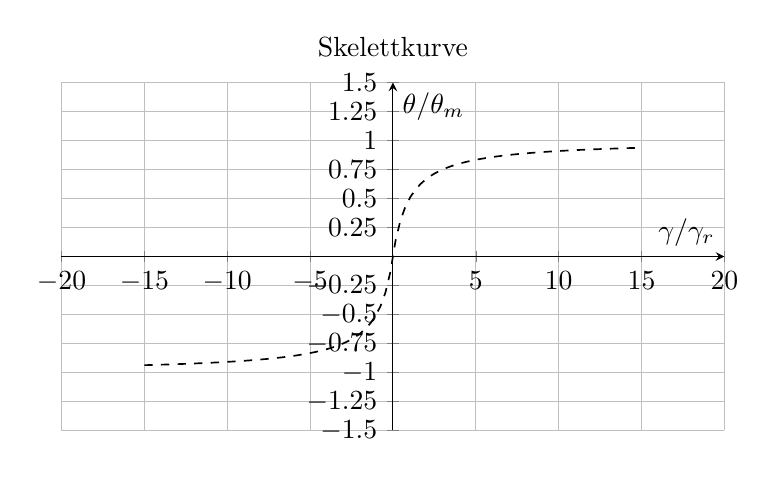
\begin{tikzpicture}
    \begin{axis}[
        title = {Skelettkurve},
        xlabel = {$\gamma / \gamma_r$},
        ylabel = {$\theta / \theta_m$},
        xmin = -20, xmax = 20,
        ymin = -1.5, ymax = 1.5,
        xtick distance = 5,
        ytick distance = 0.25,
        grid = both,
        major grid style = {lightgray},
        minor grid style = {lightgray!25},
        width = 10cm,
        height = 6 cm,
        axis x line = center,
        axis y line = center,
        domain = -15:15,
        samples = 100
        ]
    \addplot[mark=none, semithick, black, dashed]{x/(1+abs(x))};
    \end{axis}
\end{tikzpicture}
